\documentclass[11pt]{article}
\usepackage[margin=1in]{geometry}
\usepackage{amsmath,amssymb,amsthm,mathtools}
\usepackage{graphicx,booktabs,enumitem}
\usepackage[numbers,sort&compress]{natbib}
\usepackage[colorlinks=true,linkcolor=blue,citecolor=blue,urlcolor=blue]{hyperref}

\newtheorem{theorem}{Theorem}[section]
\newtheorem{proposition}[theorem]{Proposition}
\newtheorem{lemma}[theorem]{Lemma}
\newtheorem{corollary}[theorem]{Corollary}
\theoremstyle{definition}
\newtheorem{definition}[theorem]{Definition}
\newtheorem{example}[theorem]{Example}
\newtheorem{assumption}[theorem]{Assumption}
\theoremstyle{remark}
\newtheorem{remark}[theorem]{Remark}

\newcommand{\R}{\mathbb{R}}
\newcommand{\N}{\mathbb{N}}
\newcommand{\E}{\mathbb{E}}
\renewcommand{\P}{\mathbb{P}}
\newcommand{\X}{\mathsf{X}}
\newcommand{\C}{\mathcal{C}}
\newcommand{\M}{\mathcal{M}}
\newcommand{\T}{\mathbb{T}}
\newcommand{\Id}{\mathrm{Id}}
\newcommand{\dd}{\,\mathrm{d}}
\newcommand{\sgn}{\operatorname{sgn}}
\newcommand{\Wh}{\widehat W}
\newcommand{\todo}[1]{\textbf{[TODO: #1]}}

\title{Sampler-independent integrability horizons and bounded unbiased
estimators for branching representations of semilinear PDEs}
\author{[Authors to be decided]}
\date{Draft of 29 September 2026}

\begin{document}
\maketitle

\begin{abstract}
Branching (coding-tree) Monte Carlo methods represent the solution of a
semilinear parabolic PDE as the expectation of a random functional of a
marked branching diffusion. Their use is limited by integrability: beyond
a short horizon the functional ceases to have a finite variance, and the
literature provides sufficient conditions only. We show that for a fixed
tree expansion the first absolute moment of the estimator does not depend
on the sampling law (lifetime distribution, branching probabilities,
adaptive choices) and equals the minimal solution of a positive
\emph{majorant system}. Conversely, whenever this majorant is finite we
construct, from any supersolution of the majorant system, an unbiased
estimator whose output is bounded by the supersolution, and, when the
supersolution has a multiplicative slack $\vartheta>1$, whose expected
number of generated nodes is at most $\vartheta/(\vartheta-1)$ uniformly in
the horizon. In particular, the supremum over all samplers of the horizon
of finite variance equals the absolute-integrability horizon, and it is
attained with bounded output. We compute this horizon exactly for constant
data, including its endpoint behaviour, classify all-horizon integrability
on compact tori, exhibit a Fujita-type dimension threshold on $\R^d$, and
show that standard fixed-rate samplers lose finite variance strictly
earlier: for flat Allen--Cahn data at most $0.9955$ against the intrinsic
horizon $(3\pi-2\log 3)/5\approx 1.4455$, and with the uniform tuple
choice of standard implementations only $0.9955/\sqrt{d+1}$ in dimension
$d$. The node-weighted mass is sampler independent as well, which makes
the work of bounded-output sampling near the horizon exactly
$\Theta((\tau-T)^{-1})$ for constant data. Numerical experiments on
Allen--Cahn data in dimensions $1$ and $100$ confirm certified confidence
intervals up to $94\%$ of the guaranteed horizon, where fixed-rate
samplers show heavy-tailed failure.
\end{abstract}

\section{Introduction}

Probabilistic representations of semilinear PDEs by branching diffusions
go back to Skorokhod, Watanabe and McKean~\cite{McKean75}; their use as
Monte Carlo schemes free of spatial grids was developed in
\cite{HLTT14,HLOTTW19,HLT21,AC20} and extended to nonlinearities involving
derivatives of arbitrary order through \emph{coding trees}
\cite{NPP23,NPP24}. A particle carries a \emph{code} (an operator applied
to the unknown solution), lives for a random time, and branches into a
tuple of codes chosen from a mechanism derived from the chain rule. The
estimator $H$ is a product of importance weights and terminal values
along the tree, and $u=\E H$.

The central practical difficulty is integrability. The random functional
$H$ is a product over a random tree of weights that are typically larger
than one; for all but short horizons its variance is infinite, and the
Monte Carlo average then converges slowly and erratically, with heavy-tail
artefacts that masquerade as bias. Existing analyses provide sufficient
conditions: comparison with an ordinary differential equation
\cite[Thm.~3.2]{HLT21}, growth conditions on jets of the data
\cite{HP25,HP26}, or small-maturity assumptions \cite{HLOTTW19,NPP23}.
These conditions depend on the lifetime law and branching probabilities,
which are free parameters of the method, and it has remained unclear which
part of the ``short time'' restriction is intrinsic to the representation
and which part is an artefact of the sampler.

\paragraph{Contributions.} We fix the tree \emph{expansion} (the code set,
mechanism, coefficients and terminal functions) and vary everything else.
\begin{enumerate}[leftmargin=*]
\item \textbf{Sampler independence (Theorem~\ref{thm:A}).} For every
sampling law whose support covers the nonzero trees, $\E|H|=W_\Id(T,x)$,
the minimal solution of a positive majorant system obtained by replacing
every coefficient and terminal value by its absolute value. No choice of
clock or branching probabilities can extend the horizon on which $\E|H|<\infty$.
\item \textbf{Attainability with bounded output and horizon-free work
(Theorem~\ref{thm:B}).} Tilting the tree law by any supersolution
$\Wh$ of the majorant system yields an unbiased estimator with
$|H|\le\Wh_\Id(T,x)$ almost surely; a multiplicative slack $\vartheta>1$
in the supersolution inequality turns into a geometric bound on the number
of generated nodes, $\E N\le\vartheta/(\vartheta-1)$, independent of $T$.
Consequently the supremum over samplers of the finite-variance horizon
equals the absolute-integrability horizon (Corollary~\ref{cor:B1}).
Sup-norm majorants, which previously served as sufficient conditions
\cite{HLT21}, become constructive: they define the sampler.
\item \textbf{Exact horizons.} For constant data the horizon is
$\tau=\int_0^R\dd z/\Phi(z)$ with $\Phi$ the absolute Taylor series of
the nonlinearity; we identify the endpoint behaviour and the exact effect
of the slack, $W^\vartheta_\Id(t)=\vartheta|r|+Z(\vartheta^2t)$
(Theorem~\ref{thm:C}). On compact tori, all-horizon integrability holds
iff the nonlinearity is affine on the range of the data (analytic case,
Theorem~\ref{thm:D}); on $\R^d$ with small Gaussian data and quadratic
absorption it holds iff $d\ge5$ (Theorem~\ref{thm:E}).
\item \textbf{The gap for standard samplers (Proposition~\ref{prop:F}).}
With a fixed exponential clock, the second moment is governed by the
squared-jet series $\Phi_2$ and finite exactly for
$T<\lambda^{-1}\log(1+\lambda^2 p\,\tau_2)$; optimizing $\lambda$ gives
at most $0.80474\sqrt{\tau_2}$, which for flat Allen--Cahn data is
$0.9955<1.4455=\tau$. For two-term nonlinearities of degree $p$ the
attainable fraction of $\tau$ is an explicit constant tending to $0$ as
$p\to\infty$ (Remark~\ref{rem:fraction}). In dimension $d$, uniform tuple
choice multiplies the limit by $(d+1)^{-1/2}$ (Corollary~\ref{cor:uniform}),
whereas the sup-majorant tilt is dimension free
(Proposition~\ref{prop:dimfree}).
\item \textbf{Work.} The node-weighted mass $\E[N|H|]$ is also sampler
independent, which gives a lower bound on the work of any sampler with
bounded output. For constant data, sampling with output
$O(W)$ costs exactly $\Theta((\tau-T)^{-1})$ nodes near the horizon
(Corollary~\ref{cor:work}).
\end{enumerate}

\paragraph{Relation to prior work.} Zero-variance importance sampling
\cite{KM53}, Doob transforms of branching processes and Boltzmann
samplers for the trees of $Y'=\Phi(Y)$ \cite{BFS92,DFLS04} are classical,
and the cancellation behind Theorem~\ref{thm:A} is implicit in
\cite{HLTT14}. For integral equations with power nonlinearity
$\varphi=K\varphi^n+h$, branching estimators go back to Ermakov
\cite{Ermakov73,EM82}, and variance criteria through majorant equations
and ``value modelling'' (densities multiplied by the solution) were
developed by Mikhailov and coauthors \cite{Mikhailov92,Mikhailov09}; see
also \cite{RRM10} for the parabolic Cauchy problem. Medvedev and Mikhailov
\cite[\S6]{Mikhailov09} note that an ideal zero-variance version of the
nonlinear estimator had not been studied; for the \emph{collision}
estimator, where every node contributes $h$ and keeps branching, the ideal
transition density $k\varphi^n/(\varphi-h)$ generates infinite trees, and
their Theorem~4 yields zero variance only under
$1-h/\varphi<1/n$. The tilt of Section~\ref{sec:B} is value modelling in
the \emph{absorption} form, where each node chooses between a leaf and a
branch in proportion to their masses; there the ideal tilt always
produces almost surely finite trees with $|H|=W$ (Theorem~\ref{thm:B}(f)),
hence zero variance for nonnegative problems, without any condition. The
underlying principle is theirs; we do not claim it. The majorant ODE of \cite[Thm.~3.2]{HLT21} is the
spatially constant instance of our system, used there as an analysis
device for a sufficient $L^1$ condition, with the branching law chosen
independently. Branching-particle proofs of Fujita-type blow-up are
classical \cite{LMW98,CLM08}; Theorem~\ref{thm:E} applies such methods,
together with \cite{EL95}, to the moment system of a coding tree. What
we believe is new is the formulation for derivative-coded PDE trees in
which the sampler-independent horizon is an \emph{equivalence}
(Corollary~\ref{cor:B1}), the horizon-free work bound obtained from a
multiplicative slack (Theorem~\ref{thm:B}(c)), and the exact horizons and
obstructions of Theorems~\ref{thm:C}--\ref{thm:E} and
Proposition~\ref{prop:F}. \todo{check \cite{Mikhailov92} (book) for an
absorption-form ideal estimator or a slack/work bound; \cite{Mikhailov09}
checked in full text: collision form only, condition as above, work
discussed only through $n\|K\|<1$; extend the search to
neutron-transport weight windows}.

\section{Tree expansions and the majorant system}\label{sec:setting}

Let $\X$ be $\R^d$ or the flat torus $\T^d=\R^d/\mathbb{Z}^d$, let
$p_t(y,z)$ be the heat kernel of $L=\frac12\Delta$ and $P_t$ its semigroup.
Time $t$ denotes \emph{remaining} time: we consider
\begin{equation}\label{eq:pde}
\partial_t u=\tfrac12\Delta u+f(u),\qquad u(0,\cdot)=v,
\end{equation}
which is the terminal-value problem
$\partial_s u+\frac12\Delta u+f(u)=0$, $u(T)=v$, after $t=T-s$.

\begin{definition}[Expansion]
An \emph{expansion} consists of a countable code set $\C\ni\Id$,
measurable terminal functions $g_c:\X\to\R$, and for each $c\in\C$ a
finite list $\M(c)=\{(\kappa_j,(c_{j,1},\dots,c_{j,m_j}))\}_j$ of nonzero
real coefficients and code tuples.
\end{definition}

\begin{example}[Semilinear coding tree \cite{NPP23}]\label{ex:semilinear}
For \eqref{eq:pde} with $f$ smooth, take codes $\Id$, $F_k$ ($k\ge0$,
standing for $f^{(k)}(u)$) and $D_i$ ($i\le d$, standing for
$\partial_iu$), terminal functions $g_\Id=v$, $g_{F_k}=f^{(k)}(v)$,
$g_{D_i}=\partial_iv$, and
\[
\Id\to(F_0),\qquad
F_k\to(F_0,F_{k+1}),\qquad
F_k\xrightarrow{-1/2}(D_i,D_i,F_{k+2}),\qquad
D_i\to(F_1,D_i),
\]
with coefficient $1$ unless indicated. The tuples encode
$(\partial_t-L)f^{(k)}(u)=f^{(k+1)}(u)f(u)-\frac12f^{(k+2)}(u)|\nabla u|^2$
and $(\partial_t-L)\partial_iu=f'(u)\partial_iu$.
\end{example}

\paragraph{Trees and the canonical measure.}
A completed tree rooted at $(c,t,y)$ is either a \emph{leaf} with terminal
position $z\in\X$, or a \emph{branch} consisting of a lifetime
$\sigma\in(0,t)$, a branch position $z$, an index $j$, and one completed
tree rooted at $(c_{j,i},t-\sigma,z)$ for each $i\le m_j$; all children
share the position $z$. The canonical measure $\mu_{c,t,y}$ on finite
completed trees is defined recursively by
\[
\mu_{c,t,y}=\delta_{\mathrm{leaf}}\otimes p_t(y,z)\dd z
+\sum_j \mathbf 1_{(0,t)}(\sigma)\dd\sigma\otimes p_\sigma(y,z)\dd z\otimes
\bigotimes_{i}\mu_{c_{j,i},\,t-\sigma,\,z},
\]
on trees of depth at most $n$ for each $n$ (induction on $n$). The signed
weight $a(\theta)$ of a tree is the product of $g_c(z)$ over leaves and
$\kappa_j$ over branches; $N(\theta)$ denotes its number of nodes.

\begin{definition}[Majorant]
For $\vartheta\ge1$ set
$W^\vartheta_c(t,y)=\int\vartheta^{N}|a|\dd\mu_{c,t,y}\in[0,\infty]$ and
$W=W^1$. When $W_c(t,y)<\infty$ put $U_c(t,y)=\int a\dd\mu_{c,t,y}$.
\end{definition}

\begin{lemma}\label{lem:majorant}
$W^\vartheta$ is the minimal $[0,\infty]$-valued solution of
\begin{equation}\label{eq:majorant}
W^\vartheta_c(t,y)=\vartheta\Big[P_t|g_c|(y)+\sum_j|\kappa_j|\int_0^t
P_\sigma\Big[\prod_iW^\vartheta_{c_{j,i}}(t-\sigma,\cdot)\Big](y)\dd\sigma\Big].
\end{equation}
If $W_\Id(t,y)<\infty$ then $U$ satisfies the signed version of
\eqref{eq:majorant} (with $\vartheta=1$, $g_c$, $\kappa_j$) at $(\Id,t,y)$,
and at almost every state reached from it.
\end{lemma}
\begin{proof}
Tonelli's theorem applied to the recursive definition gives
\eqref{eq:majorant}. Let $W^{(n)}$ be the integral over trees of depth at
most $n$; then $W^{(n)}\uparrow W^\vartheta$, and if $V\ge0$ solves
\eqref{eq:majorant} then $W^{(n)}\le V$ by induction on $n$. The signed
statement follows by Fubini under absolute integrability.
\end{proof}

\begin{proposition}[Correspondence]\label{prop:corr}
In Example~\ref{ex:semilinear} let $f$ be a polynomial and $v\in C^2_b(\X)$.
If $W_c$ is bounded on $[0,T]\times\X$ for every code $c$, then
\eqref{eq:pde} has a unique bounded classical solution on $[0,T]$, and
$U_\Id=u$ there.
\end{proposition}
The proof (Appendix~\ref{app:corr}) is the finite-system uniqueness
argument of \cite[Thm.~3.2]{HLT21}; compare \cite[Thm.~4.2]{NPP23} and
\cite{HP25}, where integrability is assumed or derived from sufficient
conditions. In Theorem~\ref{thm:B} it suffices that the supersolution is
bounded, since $W\le\Wh$.

\section{Samplers and sampler independence}\label{sec:A}

A \emph{sampler with cemetery} for $(T,x)$ is a probability law $Q$ on
finite completed trees rooted at $(\Id,T,x)$ together with a cemetery
point $\dagger$. On a tree, the estimator is
$H=a\,\dd\mu/\dd Q$; on $\dagger$, $H=0$. We call $Q$ \emph{supported}
if $\dd Q/\dd\mu>0$ $\mu$-a.e.\ on $\{a\ne0\}$. The fixed-rate samplers of
\cite{HLOTTW19,NPP23} (exponential lifetimes of rate $\lambda$, tuple
probabilities $q_j>0$, Brownian positions) are supported samplers without
cemetery, with $H$ the familiar product of $\kappa_j/(q_j\lambda
e^{-\lambda\sigma})$ over branches and $g/e^{-\lambda t}$ over leaves.
Adaptive choices (depending on the history of the tree) are allowed; only
the joint density on complete trees enters.

\begin{theorem}[Sampler independence]\label{thm:A}
Let $W_N(T,x)=\int N|a|\dd\mu_{\Id,T,x}$. For every supported sampler,
\[
\E_Q|H|=W_\Id(T,x),\qquad \E_Q\big[N\,|H|\big]=W_N(T,x).
\]
Consequently $\E_QH^2\ge W_\Id(T,x)^2$; if $W_\Id(T,x)=\infty$ no
supported sampler of this expansion has a finite first absolute moment;
and every supported sampler with $|H|\le M$ a.s.\ satisfies
$\E_QN\ge W_N(T,x)/M$. Moreover $W_N=\lim_{\vartheta\downarrow1}
(W^\vartheta_\Id-W_\Id)/(\vartheta-1)$, and
$W_N\le W^\vartheta_\Id/(\vartheta-1)$ for every $\vartheta>1$.
\end{theorem}
\begin{proof}
For any measurable $\psi\ge0$ on trees,
$\E_Q[\psi|H|]=\int_{\{a\ne0\}}\psi|a|\frac{\dd\mu}{\dd Q}\dd Q
=\int\psi|a|\dd\mu$; take $\psi=1$ and $\psi=N$. Jensen's inequality gives
the second-moment bound, and $\E_Q[N|H|]\le M\,\E_QN$ the work bound. The
map $\vartheta\mapsto W^\vartheta_\Id=\int\vartheta^N|a|\dd\mu$ is convex
with right derivative $W_N$ at $1$ (monotone convergence of the difference
quotients $(\vartheta^N-1)/(\vartheta-1)\downarrow N$), so
$W^\vartheta_\Id\ge W_\Id+(\vartheta-1)W_N$.
\end{proof}

\section{Tilted samplers}\label{sec:B}

\begin{definition}\label{def:super}
Let $\vartheta\ge1$ and let $h_c\ge|g_c|$ be measurable envelopes. A
measurable $\Wh:\C\times(0,T]\times\X\to[0,\infty]$ is a
\emph{$\vartheta$-supersolution} if for all $(c,t,y)$
\begin{equation}\label{eq:super}
\Wh_c(t,y)\ge\vartheta\Big[L_c(t,y)+\sum_j|\kappa_j|B_{c,j}(t,y)\Big],
\quad L_c=P_th_c,\quad
B_{c,j}(t,y)=\int_0^t\!\!\int p_\sigma(y,z)\prod_i\Wh_{c_{j,i}}(t-\sigma,z)\dd z\dd\sigma,
\end{equation}
with the convention $0\cdot\infty=0$.
\end{definition}

\paragraph{The tilted sampler.} Define a recursive procedure
$S(c,t,y)$ with values in $[-1,1]$:
\begin{enumerate}[leftmargin=*]
\item with probability $L_c/\Wh_c$: leaf; draw $z$ with density
$p_t(y,z)h_c(z)/L_c(t,y)$ and return $g_c(z)/h_c(z)$;
\item with probability $|\kappa_j|B_{c,j}/\Wh_c$: branch $j$; draw
$(\sigma,z)$ with density
$p_\sigma(y,z)\prod_i\Wh_{c_{j,i}}(t-\sigma,z)/B_{c,j}(t,y)$ and return
$\sgn(\kappa_j)\prod_iS(c_{j,i},t-\sigma,z)$, evaluating the children
one after another;
\item otherwise: kill, i.e.\ stop the whole computation and output $0$.
\end{enumerate}
The estimator is $H=\Wh_\Id(T,x)\,S(\Id,T,x)$ (and $H=0$ if
$\Wh_\Id(T,x)=0$).

\begin{theorem}\label{thm:B}
Let $\Wh$ be a $\vartheta$-supersolution with $\Wh_\Id(T,x)<\infty$.
\begin{enumerate}[label=(\alph*),leftmargin=*]
\item Almost surely every visited state has $0<\Wh<\infty$.
\item $|H|\le\Wh_\Id(T,x)$ almost surely.
\item If $\vartheta>1$, the number $N_{\rm gen}$ of generated nodes satisfies
$\P(N_{\rm gen}>n)\le\vartheta^{-n}$; in particular
$\E N_{\rm gen}\le\vartheta/(\vartheta-1)$.
\item If the procedure stops almost surely (always when $\vartheta>1$), then
$W_\Id(T,x)\le\Wh_\Id(T,x)$, the sampler is supported, and $\E H=U_\Id(T,x)$.
\item $\E H^2\le\Wh_\Id(T,x)\,W^{(h)}_\Id(T,x)$, where $W^{(h)}$ is the
majorant with $h$ in place of $|g|$; with $h=|g|$ equality holds, and
$\E H^2\le(\Wh_\Id/W_\Id)\inf_Q\E_QH^2$ over supported samplers $Q$.
\item If $W_\Id(T,x)<\infty$, the choice $\Wh=W$, $h=|g|$, $\vartheta=1$
never kills, stops almost surely, and gives $|H|=W_\Id(T,x)$ a.s.
\end{enumerate}
\end{theorem}

\begin{proof}
(a) At a state with $\Wh_c\in(0,\infty)$ the branch density has total mass
$B_{c,j}\le\Wh_c/\vartheta<\infty$, so the set of $(\sigma,z)$ at which
some child has $\Wh=\infty$ while the product is positive is null, and
where the product vanishes the density vanishes. The root is covered by
assumption.
(b) By induction on the finite tree, $S\in[-1,1]$.
(c) Nodes are generated one at a time. Conditionally on everything
generated before, the current node is killed with probability
$1-(L_c+\sum_j|\kappa_j|B_{c,j})/\Wh_c\ge1-\vartheta^{-1}$ by
\eqref{eq:super}. Generating an $(n+1)$st node requires $n$ non-kills.
(d) The $Q$-density of a completed, non-killed tree $\theta$ is a
product of step probabilities and conditional densities: a leaf
contributes $p_th_c/\Wh_c$, a branch contributes
$|\kappa_j|p_\sigma\prod_i\Wh_{c_{j,i}}/\Wh_c$. Every non-root $\Wh$
appears once in a numerator and once in a denominator, hence
\[
\frac{\dd Q}{\dd\mu}(\theta)=\frac{|a_h(\theta)|}{\Wh_\Id(T,x)},\qquad
a_h=\prod_{\rm branches}\kappa_j\prod_{\rm leaves}h_c(z),
\]
which is positive where $a\ne0$. On $\theta$,
$H=\Wh_\Id\prod\sgn(\kappa_j)\prod g_c/h_c=a\,\dd\mu/\dd Q$. Hence
$\int|a|\dd\mu\le\int|a_h|\dd\mu=\Wh_\Id\,Q(\text{completed})\le\Wh_\Id$,
and, the procedure stopping a.s., $\E H=\int a\dd\mu=U_\Id(T,x)$.
(e) $\E H^2\le\Wh_\Id^2Q(\text{completed})=\Wh_\Id\int|a_h|\dd\mu$, with
equality if $|g/h|=1$; combine with Theorem~\ref{thm:A}.
(f) With $\Wh=W$, \eqref{eq:super} holds with equality by
Lemma~\ref{lem:majorant}, so no kill occurs, and completed trees have
$Q$-mass $\int|a|\dd\mu/W_\Id=1$.
\end{proof}

\begin{corollary}[Sampler-independent horizon]\label{cor:B1}
For fixed $(T,x)$ the following are equivalent: (i) some supported sampler
has $\E|H|<\infty$; (ii) every supported sampler has $\E|H|<\infty$;
(iii) $W_\Id(T,x)<\infty$; (iv) some supported sampler that stops almost
surely has $|H|=W_\Id(T,x)$ a.s. In particular the supremum over supported
samplers of the horizons of finite variance equals the horizon of
absolute integrability, and it is attained with bounded output.
\end{corollary}

\begin{corollary}[Horizon-free work]\label{cor:B2}
If $W^\vartheta_\Id(T,x)<\infty$ for some $\vartheta>1$, tilting by
$W^\vartheta$ with $h=|g|$ gives an unbiased estimator with
$|H|\le W^\vartheta_\Id(T,x)$, $\E H^2=W^\vartheta_\Id(T,x)W_\Id(T,x)$ and
$\E N_{\rm gen}\le\vartheta/(\vartheta-1)$.
\end{corollary}
\begin{proof}
$W^\vartheta$ satisfies \eqref{eq:super} with equality by
Lemma~\ref{lem:majorant}; apply Theorem~\ref{thm:B}.
\end{proof}

\begin{remark}[Work--output trade-off]\label{rem:tradeoff}
By Theorem~\ref{thm:A}, every supported sampler with output bound $M$
needs $\E N\ge W_N/M$, so the product of the output bound and the
expected work is at least $W_N$, whatever the sampler. The tilt of
Corollary~\ref{cor:B2} achieves $M\,\E N\le W^\vartheta_\Id\,
\vartheta/(\vartheta-1)$. Section~\ref{sec:explicit} shows that for
constant data both sides are of the same order near the horizon.
\end{remark}

\paragraph{Spatially constant supersolutions.} Take constant envelopes
$h_c\equiv\ell_c\ge\sup|g_c|$. If $\Wh_c(t)$ does not depend on $y$ and
solves
\begin{equation}\label{eq:supode}
\Wh_c(t)=\vartheta\Big[\ell_c+\sum_j|\kappa_j|\int_0^t\prod_i\Wh_{c_{j,i}}(s)\dd s\Big],
\end{equation}
then it is a $\vartheta$-supersolution, since $\int p_\sigma(y,z)\dd z=1$.
The branch step then factorizes: $j$ and the children's remaining time
$s=t-\sigma$ are drawn from $|\kappa_j|\prod_i\Wh_{c_{j,i}}(s)$ on
$(0,t)$, and $z=y+\sqrt\sigma\,\xi$ with a standard Gaussian $\xi$; a leaf
uses $z=y+\sqrt t\,\xi$ and returns $g_c(z)/\ell_c$. For polynomial $f$ of
degree $m$ in Example~\ref{ex:semilinear}, \eqref{eq:supode} is a finite
ODE system in the codes $\Id,F_0,\dots,F_m,D_1,\dots,D_d$. For $\vartheta=1$
it is the sup-majorant ODE of \cite[(3.10)]{HLT21} (there without gradient
codes), which yields a sufficient integrability condition; here it defines
the sampler.

\begin{proposition}[Dimension-free sup majorant]\label{prop:dimfree}
In Example~\ref{ex:semilinear} on $\R^d$ or $\T^d$ with polynomial $f$,
let $\ell_{D_i}\ge\sup|\partial_iv|$ and $\ell_D=(\sum_i\ell_{D_i}^2)^{1/2}$.
The minimal solution of \eqref{eq:supode} satisfies
$\Wh_{D_i}=(\ell_{D_i}/\ell_D)\Wh_D$, where $(\Wh_\Id,\Wh_{F_k},\Wh_D)$
solves the one-dimensional system with $\ell_D$ in place of
$\sup|v'|$. Consequently the guaranteed horizon, the output bound and
the work bound $\vartheta/(\vartheta-1)$ depend on $d$ only through
$\ell_D$, and the tilted sampler chooses the tuple $(D_i,D_i,F_{k+2})$
with direction $i$ drawn with probability $\ell_{D_i}^2/\ell_D^2$.
\end{proposition}
\begin{proof}
The equations for $D_i$ are $\Wh_{D_i}=\vartheta[\ell_{D_i}+\int_0^t
\Wh_{F_1}\Wh_{D_i}]$, linear in $\ell_{D_i}$ given $\Wh_{F_1}$, so the
ansatz is consistent; and $\frac12\sum_i\Wh_{D_i}^2=\frac12\Wh_D^2$ in
the equations for $F_k$. Minimal solutions are unique for this finite
locally Lipschitz system up to blow-up. The branch mass of the tuple
$(D_i,D_i,F_{k+2})$ is the fraction $\ell_{D_i}^2/\ell_D^2$ of the
aggregated one, and the $D_i$ nodes have the same leaf and branch
probabilities as the aggregated code, with leaf factor
$\partial_iv(z)/\ell_{D_i}$.
\end{proof}

For data depending on one direction, $v(x)=\psi(a\cdot x)$ with $|a|=1$,
one has $\ell_D=\sup|\psi'|$ for every $d$; the same aggregation shows that
the \emph{exact} majorant $W$ of the $d$-dimensional expansion equals the
one-dimensional one, so the intrinsic horizon does not depend on $d$.

\begin{corollary}[Certified confidence intervals]\label{cor:hoeffding}
Under Theorem~\ref{thm:B}(d), the mean $\bar H_n$ of $n$ independent
copies satisfies, by Hoeffding's inequality,
$\P\big(|\bar H_n-U_\Id(T,x)|\ge\Wh_\Id(T,x)\sqrt{2\log(2/\alpha)/n}\big)\le\alpha$.
\end{corollary}

\begin{remark}[Implementation]\label{rem:impl}
Our implementation tabulates the solution of \eqref{eq:supode} as a
nondecreasing step function on an adaptive grid and computes every
probability and density in the procedure from that same step function.
Unbiasedness is then exact for the implemented sampler irrespective of the
ODE error; only the slack is affected, and it is verified on the grid as
$\vartheta_{\rm eff}=\min_{c,i}\Wh_c(s_i)/(\ell_c+\sum_j|\kappa_j|\int_0^{s_i}\prod\Wh)$
(the worst case in each cell is its right endpoint).
\end{remark}

\section{Explicit horizons}\label{sec:explicit}

\subsection{Constant data}

Let $v\equiv r$ in Example~\ref{ex:semilinear}, $a_k=|f^{(k)}(r)|$,
$\Phi(z)=\sum_{k\ge0}a_kz^k/k!$ with radius of convergence
$R\in[0,\infty]$, and $Z$ the solution of $Z'=\Phi(Z)$, $Z(0)=0$.

\begin{theorem}[Exact horizon]\label{thm:C}
Assume $a_0>0$ and put $\tau=\int_0^R\dd z/\Phi(z)$. Then
$W_{F_k}(t)=\Phi^{(k)}(Z(t))$ and $W_\Id(t)=|r|+Z(t)$ for $t<\tau$;
$W_\Id(\tau)=|r|+R$ if $\tau<\infty$; and $W_\Id(t)=\infty$ for $t>\tau$.
Moreover $W^\vartheta_{F_k}(t)=\vartheta\Phi^{(k)}(Z(\vartheta^2t))$ and
$W^\vartheta_\Id(t)=\vartheta|r|+Z(\vartheta^2t)$, so for every $T<\tau$
and $1<\vartheta<\sqrt{\tau/T}$ Corollary~\ref{cor:B2} applies with
$|H|\le\vartheta|r|+Z(\vartheta^2T)$ and $\E N_{\rm gen}\le\vartheta/(\vartheta-1)$.
If $a_0=0$ then $W_\Id\equiv|r|$.
\end{theorem}

\begin{proof}
Every tree containing a gradient code has a $D$-leaf (the $D$-chain
$D\to(F_1,D)$ ends in a leaf with $g_D=0$), so only the codes $F_k$ and
$\Id$ contribute, and \eqref{eq:majorant} reduces to $V_k(t)=a_k+\int_0^t
V_0V_{k+1}$, $W_\Id(t)=|r|+\int_0^tV_0$. Truncate the jet at order $n$
(set $a_k=0$ for $k>n$): this is a nonnegative truncation of tree weights,
monotone in $n$ and exhausting all finite trees. The truncated system has
the minimal solution $V_k=\Phi_n^{(k)}(Z_n)$ with $Z_n'=\Phi_n(Z_n)$,
$Z_n(0)=0$, as one checks by differentiation; finite-dimensional
uniqueness identifies it with the tree sum up to its explosion time
$\tau_n=\int_0^\infty\dd z/\Phi_n$, after which the tree sum is infinite
by monotonicity in $t$. As $n\to\infty$, $\Phi_n\uparrow\Phi$ on $[0,R)$
and $\Phi_n\uparrow\infty$ beyond $R$; monotone convergence gives
$\tau_n\downarrow\tau$ and $Z_n\uparrow Z$ on $[0,\tau)$. For $t>\tau$ some
$\tau_n<t$, whence $W_\Id(t)=\infty$. At $t=\tau$, grouping trees by the
number of internal nodes shows $W_\Id(t)-|r|$ is a power series in $t$
with nonnegative coefficients, so its value at $\tau$ is the left limit
$R$. For $\vartheta$: $V_k=\vartheta\Psi_k(\vartheta^2t)$ solves
$V_k=\vartheta[a_k+\int_0^tV_0V_{k+1}]$ iff $\Psi$ solves the case
$\vartheta=1$, and minimality is preserved by the scaling; then
$W^\vartheta_\Id(t)=\vartheta|r|+\vartheta\int_0^tV_0=\vartheta|r|+Z(\vartheta^2t)$.
If $a_0=0$ every tree through $F_0$ has a zero $F_0$-leaf or a zero
$D$-leaf.
\end{proof}

\begin{corollary}[Work near the horizon]\label{cor:work}
In Theorem~\ref{thm:C}, $W_N(T)=|r|+2T\,\Phi(Z(T))$ for $T<\tau$. If
$\Phi$ is a polynomial of degree $p\ge2$, then as $T\uparrow\tau$:
\begin{enumerate}[label=(\roman*),leftmargin=*]
\item every supported sampler with $|H|\le C\,W_\Id(T)$ a.s.\ has
$\E N\ge(1+o(1))\,\dfrac{2\tau}{C(p-1)(\tau-T)}$;
\item the tilt by $W^\vartheta$ with $\vartheta^2=(\tau+T)/(2T)$ has
$|H|\le(2^{1/(p-1)}+o(1))\,W_\Id(T)$ and $\E N\le(4\tau+o(1))/(\tau-T)$.
\end{enumerate}
Hence unbiased sampling with output bounded by a constant multiple of
$W_\Id$ costs $\Theta((\tau-T)^{-1})$ expected nodes per sample.
\end{corollary}
\begin{proof}
$W_N=\partial_\vartheta[\vartheta|r|+Z(\vartheta^2T)]_{\vartheta=1}
=|r|+2TZ'(T)$ by Theorem~\ref{thm:A}. Let $\Phi$ have leading term
$a_pz^p/p!$. From $\int_{Z(t)}^\infty\dd z/\Phi=\tau-t$ one gets
$Z(t)^{p-1}\sim p!/(a_p(p-1)(\tau-t))$ and
$\Phi(Z)/Z\sim1/((p-1)(\tau-t))$, so $W_N/W_\Id\sim2\tau/((p-1)(\tau-T))$,
and (i) follows from Theorem~\ref{thm:A}. For (ii),
$\tau-\vartheta^2T=(\tau-T)/2$, so $W^\vartheta_\Id=\vartheta|r|+
Z(\tau-(\tau-T)/2)\sim2^{1/(p-1)}Z(T)$, and
$\vartheta/(\vartheta-1)\sim2/(\vartheta^2-1)=4T/(\tau-T)$.
\end{proof}

\begin{example}\label{ex:ac}
Allen--Cahn $f(u)=u-u^3$, $r=\frac12$: $\Phi(z)=(z+\frac32)(z^2+\frac14)$,
$\tau=(3\pi-2\log3)/5\approx1.44551$. For $f=\sin$, $r=\pi/2$: $\Phi=\cosh$,
$\tau=\pi/2$ and $W_\Id(\tau)=\infty$, while the ODE solution
$2\arctan e^t$ is global. For $f(y)=(1+y^2)^{-1}$, $r=0$:
$\Phi(z)=(1-z^2)^{-1}$, $R=1$, $\tau=2/3$ and $W_\Id(2/3)=1<\infty$, but
$W_\Id(t)=\infty$ for every $t>2/3$.
\end{example}

\subsection{Fixed-rate samplers}

\begin{proposition}\label{prop:F}
In the setting of Theorem~\ref{thm:C}, consider the fixed-rate sampler
with exponential lifetimes of rate $\lambda>0$ and probability $p\in(0,1]$
on the tuple $(F_0,F_{k+1})$ (the other tuple carries zero weight). Let
$\Phi_2(z)=\sum_ka_k^2z^k/k!$ and $\tau_2=\int_0^{R_2}\dd z/\Phi_2$. If
$\Phi_2$ is a polynomial of degree at least two, then $\E H^2<\infty$ iff
\[
T<T_2(\lambda,p)=\lambda^{-1}\log\big(1+\lambda^2p\,\tau_2\big),
\qquad
\sup_{\lambda>0}T_2(\lambda,p)=K\sqrt{p\,\tau_2},\quad
K=\max_{z>0}\frac{\log(1+z)}{\sqrt z}\approx0.804743.
\]
For Example~\ref{ex:ac}, $\tau_2=1.530121\ldots$ and
$\sup_{\lambda,p}T_2=0.99545<\tau$.
\end{proposition}

\begin{proof}
A leaf at remaining time $t$ has weight $g/e^{-\lambda t}$, a branch
$\kappa/(p\lambda e^{-\lambda\sigma})$. Conditioning on the first event,
the second moments $M_c$ satisfy
$M_{F_k}(t)=a_k^2e^{\lambda t}+(p\lambda)^{-1}\int_0^te^{\lambda\sigma}
M_{F_0}(t-\sigma)M_{F_{k+1}}(t-\sigma)\dd\sigma$ (minimal solutions, as in
Lemma~\ref{lem:majorant}). Since the tuples are binary, writing
$M_{F_k}=e^{\lambda t}z_k$ and changing time to
$\theta=(e^{\lambda t}-1)/\lambda^2$ (so $\dd\theta=\lambda^{-1}e^{\lambda
t}\dd t$) gives
\[
z_k(\theta)=a_k^2+p^{-1}\int_0^\theta z_0\,z_{k+1}\dd\theta'.
\]
Introduce $s$ by $\dd s/\dd\theta=z_0$, $s(0)=0$. Then
$\dd z_k/\dd s=z_{k+1}/p$, so $z_k=\Phi_2^{(k)}(s/p)$ (a finite sum), and
$v=s/p$ solves $\dd v/\dd\theta=\Phi_2(v)/p$. Hence the $F$-moments are
finite exactly for $\theta<\theta_*=p\,\tau_2$ and diverge as
$\theta\uparrow\theta_*$; as in Theorem~\ref{thm:C} the finite polynomial
system identifies the minimal solution, and monotonicity in $t$ gives
divergence after $\theta_*$. The single-child $\Id$ code has
$M_\Id(t)=e^{\lambda t}\big[r^2+\lambda^{-1}\int_0^tz_0\dd t'\big]$ and
$\int z_0\dd t'=\int\lambda e^{-\lambda t'}\dd s\ge
\lambda(1+\lambda^2\theta_*)^{-1}s\to\infty$ as $\theta\uparrow\theta_*$,
so the root diverges at the same time. Solving
$\theta_*=(e^{\lambda T}-1)/\lambda^2$ gives $T_2$, and with
$z=\lambda^2p\tau_2$, $T_2=\sqrt{p\tau_2}\log(1+z)/\sqrt z$, maximized
at the unique root of $2z/(1+z)=\log(1+z)$, $z_*\approx3.9215$.
\end{proof}

\begin{corollary}[Uniform tuples in dimension $d$]\label{cor:uniform}
In $\R^d$, the mechanism of Example~\ref{ex:semilinear} gives each $F_k$
the $1+d$ tuples $(F_0,F_{k+1})$ and $(D_i,D_i,F_{k+2})$, $i\le d$. For
constant data the latter carry zero weight, so a fixed-rate sampler with
uniform tuple choice, as in \cite{NPP23,NPP24}, is the case
$p=1/(d+1)$ of Proposition~\ref{prop:F}: its variance is finite exactly for
$T<\lambda^{-1}\log(1+\lambda^2\tau_2/(d+1))$, and
$\sup_\lambda T_2=K\sqrt{\tau_2/(d+1)}$. For flat Allen--Cahn data in
$d=100$ this is $0.0990$ ($0.0294$ at $\lambda=2$), against the
dimension-independent intrinsic horizon $1.4455$.
\end{corollary}

\begin{remark}\label{rem:fraction}
For a two-term series $\Phi(z)=a_0+a_pz^p/p!$ the substitution
$z=(a_0p!/a_p)^{1/p}u$ gives $\tau=a_0^{-1}(a_0p!/a_p)^{1/p}I_p$ and
$\tau_2=a_0^{-2}(a_0^2p!/a_p^2)^{1/p}I_p$, $I_p=\int_0^\infty\dd u/(1+u^p)
=\frac{\pi/p}{\sin(\pi/p)}$. Hence the best fixed-rate sampler reaches the
fraction
\[
\frac{\sup_{\lambda,p}T_2}{\tau}=K\,(p!)^{-1/(2p)}\,I_p^{-1/2},
\]
independently of $a_0,a_p$: $0.540$ for $p=2$, $0.543$ for $p=3$, $0.454$
for $p=6$, $0.375$ for $p=10$, and $\sim K\sqrt{e/p}\to0$ as $p\to\infty$
(checked against quadrature to $10^{-15}$). Fixed-rate samplers thus lose
a fraction of the intrinsic horizon that grows with the degree of the
nonlinearity, whereas Theorem~\ref{thm:B} attains all of it.
\end{remark}

\subsection{Compact tori}

\begin{theorem}\label{thm:D}
Let $\X=\T^d$, $v$ smooth and nonconstant, $f$ real-analytic on an open
interval containing $v(\X)$, in Example~\ref{ex:semilinear}. Then
$W_\Id(T,x)<\infty$ for every $T$ and $x$ iff $f$ is affine on $v(\X)$.
More generally, for smooth $f$ and smooth $v$, all-horizon integrability
holds iff $f(v)\equiv0$ or $f^{(p)}(v)\equiv0$ for all $p\ge2$; if
$f(v)\not\equiv0$ and $f^{(p)}(v)\not\equiv0$, then with
$\eta_q=\min_xP_{t_0}|f^{(q)}(v)|(x)>0$,
\[
W_\Id(T,x)=\infty\quad\text{for all }x\text{ and }
T\ge t_0+\tfrac{p}{p-1}\,\eta_0^{-(p-1)/p}\,(p!/\eta_p)^{1/p}.
\]
\end{theorem}

\begin{proof}[Proof of the obstruction]
Positivity of the heat kernel on the compact torus makes $\eta_0,\eta_p$
positive. Split the time integral in \eqref{eq:majorant} at $t_0$, drop
the (nonnegative) part before $t_0$ and all tuples except the
coefficient-one chain $F_k\to(F_0,F_{k+1})$. The functions
$A_k(s)=\inf_xW_{F_k}(t_0+s,x)$ satisfy $A_k(s)\ge\eta_k\mathbf1_{k\in\{0,p\}}
+\int_0^sA_0A_{k+1}$ for $k<p$ and $A_p\ge\eta_p$, since
$P_{t_0+s}|g|=P_s(P_{t_0}|g|)\ge\min P_{t_0}|g|$. Comparison with the
finite system $V_k'=V_0V_{k+1}$ ($k<p$), $V_p=\eta_p$ gives
$A_0\ge V_0=\eta_0+(\eta_p/p!)Z^p$ with $Z'=V_0$, $Z(0)=0$, which
explodes before $\int_0^\infty\dd z/(\eta_0+\eta_pz^p/p!)$; splitting this
integral at $(\eta_0p!/\eta_p)^{1/p}$ gives the displayed bound. The
comparison is carried out on finite Picard iterates, so no infinite
moment is differentiated; $W_\Id\ge\int_0^T P_{T-s}W_{F_0}(s)\dd s$
transfers divergence to the root.
\end{proof}
\begin{proof}[Proof of sufficiency]
See Appendix~\ref{app:D}.
\end{proof}

\subsection{A Fujita-type threshold on $\R^d$}

\begin{theorem}\label{thm:E}
Let $\X=\R^d$, $f(u)=-u^2$ and $v=\varepsilon e^{-|x|^2}$ with
$0<\varepsilon\le1/32$. Then $W_\Id(T,x)<\infty$ for all $T,x$ iff
$d\ge5$. For $d\ge5$,
$W_\Id(t,x)\le(\varepsilon+C\varepsilon^2t)G(t,x)$ with
$G(t,x)=(1+t)^{-d/2}e^{-|x|^2/(2(1+t))}$, $C=2+32d/(d-2)$, and
Theorem~\ref{thm:B} applies with the supersolution
$(aG,bG,\delta G,(\varepsilon+C\varepsilon^2t)G)$ defined below, for every
horizon.
\end{theorem}

\begin{proof}[Proof for $d\ge5$]
Write $A,B,D_i$ for the majorants of $F_0,F_1,D_i$ ($W_{F_2}=2$, higher codes
vanish). Then \eqref{eq:majorant} is the mild form of
$(\partial_t-L)A=AB+\sum_iD_i^2$, $(\partial_t-L)B=2A$,
$(\partial_t-L)D_i=BD_i$, $(\partial_t-L)W_\Id=A$ with data
$v^2,2v,|\partial_iv|,v$. With $w(t)=(1+t)^{-d/2}$ one has
$(\partial_t-L)G=0$, $G^2\le wG$, $I_0=\int_0^\infty w=2/(d-2)\le2/3$,
$I_1=\int_0^\infty tw=4/((d-2)(d-4))\le4/3$. Put
$b(t)=2\varepsilon+2C\varepsilon^2t$, $J(t)=\int_0^tbw$,
$\delta(t)=2\varepsilon e^{J(t)}$ and
$a(t)=\varepsilon^2+C\varepsilon^2J(t)+4d\varepsilon^2e^{2J(\infty)}\int_0^tw$.
Then $J(\infty)\le107/576<1/4$, $a\le\frac34C\varepsilon^2$,
and $a'\ge w(ab+d\delta^2)$, $b'\ge2a$, $\delta'=wb\delta$; since each
product contributes $G^2\le wG$, $(aG,bG,\delta G)$ is a supersolution
dominating the data ($v\le\varepsilon G(0)$, $v^2\le\varepsilon^2G(0)$,
$|\partial_iv|\le2\varepsilon G(0)$).
\end{proof}
\begin{proof}[Proof for $d\le4$]
See Appendix~\ref{app:E}. The reduced system is a mixed-exponent
system in the scope of \cite{EL95}; the appendix gives a self-contained
argument with explicit horizons.
\end{proof}

\section{Numerical experiments}\label{sec:numerics}

All experiments use Example~\ref{ex:semilinear} in $d=1$ with
$f(u)=u-u^3$, the spatially constant supersolution \eqref{eq:supode}, and
pure-Python samplers; the code is available at \todo{repository}.

\paragraph{Flat data.} For $v\equiv\frac12$ the tabulated bound agrees
with $\vartheta/2+Z(\vartheta^2T)$ to the printed digits at
$T=0.5,0.9,1.2$. At $T=1.4$ ($96.9\%$ of $\tau$, beyond every fixed-rate
sampler by Proposition~\ref{prop:F}), $\vartheta=1.004$ and $1.6\times10^6$
samples give $0.917704\pm0.002741$ against the exact value $0.919628$,
with $|H|\le3.847$ and about $33$ nodes per sample. The sampler-independent
identity $\E[N|H|]=W_N=\frac12+2T\Phi(Z(T))$ of Theorem~\ref{thm:A} is
reproduced within one standard error ($2\times10^5$ samples): $2.226\pm
0.007$ vs $2.219$ at $T=0.9$, $7.487\pm0.030$ vs $7.512$ at $T=1.2$,
$101.5\pm0.4$ vs $101.85$ at $T=1.4$; the measured $\E N$ ($2.51$, $6.21$,
$32.9$) lies between the lower bound $W_N/M$ ($1.75$, $3.61$, $26.5$) and
$\vartheta/(\vartheta-1)$ ($11$, $21$, $251$).

\paragraph{Periodic data.} For $v=\frac12+0.02\sin(2\pi x)$ on $\T^1$ the
exact sup envelopes give the guaranteed horizon $\tau_{\sup}=1.28237$.
Figure~\ref{fig:periodic} and Table~\ref{tab:periodic} compare the tilted
sampler with fixed-rate samplers (rates $1$ and $2$, uniform tuples) at
$x=\frac14$, $2\times10^5$ samples each, against a pseudo-spectral
reference (256 modes, Strang splitting with exact reaction flow; step
halving changes it by less than $1.4\times10^{-11}$). The tilted estimates
lie within $1.8$ standard errors of the reference and inside the certified
Hoeffding intervals at every $T$. The fixed-rate samplers exhibit
heavy tails from $T\approx0.8$ on: the largest $0.1\%$ of samples carry
up to $18\%$ of $\sum|H|$, maximal $|H|$ reach $10^4$, and at $T=1.2$ the
rate-one estimate deviates by $3.2$ of its own standard errors.

\begin{table}[t]
\centering\small
\begin{tabular}{@{}cccccc@{}}
\toprule
$T$ & reference & tilted (s.e.) & Hoeffding 95\% & rate 1 (s.e.), $\max|H|$ & rate 2 (s.e.), $\max|H|$\\
\midrule
0.5 & 0.68946 & 0.68884 (0.00051) & 0.0046 & 0.68905 (0.00075), 23 & 0.68932 (0.00127), 10\\
0.8 & 0.78916 & 0.78716 (0.00112) & 0.0061 & 0.78626 (0.00411), 665 & 0.79102 (0.00267), 108\\
1.0 & 0.84334 & 0.84247 (0.00186) & 0.0081 & 0.82450 (0.01567), 2630 & 0.85240 (0.00873), 854\\
1.1 & 0.86632 & 0.87069 (0.00253) & 0.0104 & 0.91542 (0.02545), 4650 & 0.79822 (0.05822), 11200\\
1.2 & 0.88660 & 0.88633 (0.00407) & 0.0178 & 0.94836 (0.01935), 1420 & 0.93548 (0.06933), 9330\\
\bottomrule
\end{tabular}
\caption{Periodic Allen--Cahn, $v=\frac12+0.02\sin(2\pi x)$, $x=\frac14$.
Tilted sampler with $\vartheta=1.02$ ($1.0169$ at $T=1.2$); mean nodes per
sample $1.5,2.2,3.9,6.4,16.4$. Fixed-rate standard errors at $T\ge1$ are
not reliable (possibly infinite variance).}
\label{tab:periodic}
\end{table}

\begin{figure}[t]
\centering
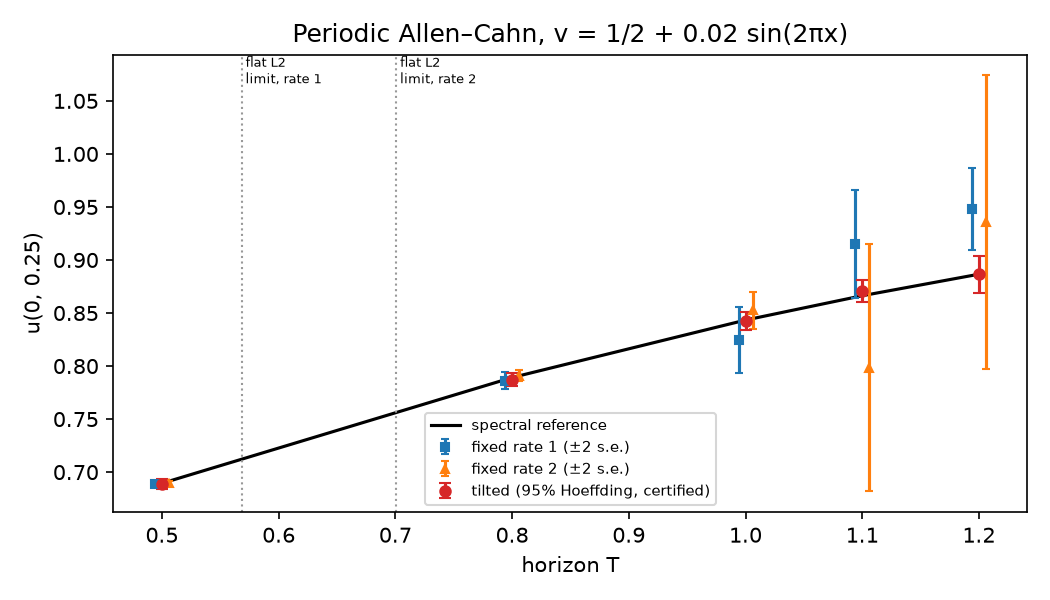
\includegraphics[width=0.8\textwidth]{tilted_long_horizon.png}
\caption{Estimates of $u(0,\frac14)$ against the horizon. Vertical lines:
finite-variance limits of the fixed-rate samplers for the flat data
(Proposition~\ref{prop:F}).}
\label{fig:periodic}
\end{figure}

\paragraph{Dimension $100$.} For $v(x)=\frac12+0.02\sin(2\pi a\cdot x)$
on $\R^{100}$ with $a=(1,\dots,1)/10$, the exact solution is the
one-dimensional periodic solution evaluated at $a\cdot x$, since $a\cdot B$
is a standard Brownian motion; all samplers nevertheless simulate the
100-dimensional tree. By Proposition~\ref{prop:dimfree} the tilted
sampler has the same guaranteed horizon $1.28237$ as in one dimension.
We compare it at $x_0=a/4$ with fixed-rate samplers ($\lambda=2$) using
uniform tuples over the $101$ tuples of each $F_k$ code, and a tuned
main-label probability $0.95$ (Table~\ref{tab:hd}, Figure~\ref{fig:hd},
$10^5$ samples each). The flat-data limits of Corollary~\ref{cor:uniform}
are $0.029$ (uniform) and $0.96$ (tuned). The uniform sampler is heavy-tailed
from $T=0.6$ ($\max|H|=5876$) and wrong by $8.8$ and $16$ of its standard
errors at $T=1.0$ and $1.2$; the tuned sampler holds to $T=1.0$ and turns
heavy-tailed at $T=1.2$ ($\max|H|=2030$); the tilted sampler's certified
intervals cover the reference at every $T$. Independent repetitions of
the tilted runs (ten seeds, up to $2\times10^6$ samples) give pooled
$z$-scores $-0.03$, $-0.25$, $-0.39$, $+1.56$ at $T=0.02,0.1,1.0,1.2$.

\begin{table}[t]
\centering\small
\begin{tabular}{@{}ccccc@{}}
\toprule
$T$ & reference & tilted (s.e.), nodes & uniform $\lambda=2$ (s.e.), $\max|H|$ & tuned $\lambda=2$ (s.e.), $\max|H|$\\
\midrule
0.1 & 0.54072 & 0.54128 (0.00025), 1.07 & 0.54114 (0.00052), 4.0 & 0.54056 (0.00050), 0.64\\
0.3 & 0.61476 & 0.61510 (0.00040), 1.23 & 0.61643 (0.00120), 8.9 & 0.61465 (0.00108), 0.95\\
0.6 & 0.72479 & 0.72566 (0.00094), 1.64 & 0.68449 (0.05882), 5876 & 0.72528 (0.00214), 3.7\\
1.0 & 0.84334 & 0.83839 (0.00265), 3.90 & 0.93657 (0.01059), 853 & 0.84578 (0.00503), 62\\
1.2 & 0.88660 & 0.86767 (0.00576), 16.6 & 1.03702 (0.00934), 190 & 0.88252 (0.02646), 2030\\
\bottomrule
\end{tabular}
\caption{Allen--Cahn in $d=100$, $x_0=a/4$, one seed per column; Hoeffding
95\% half-widths of the tilted sampler: $0.0049$, $0.0057$, $0.0071$,
$0.0115$, $0.0252$.}
\label{tab:hd}
\end{table}

\begin{figure}[t]
\centering
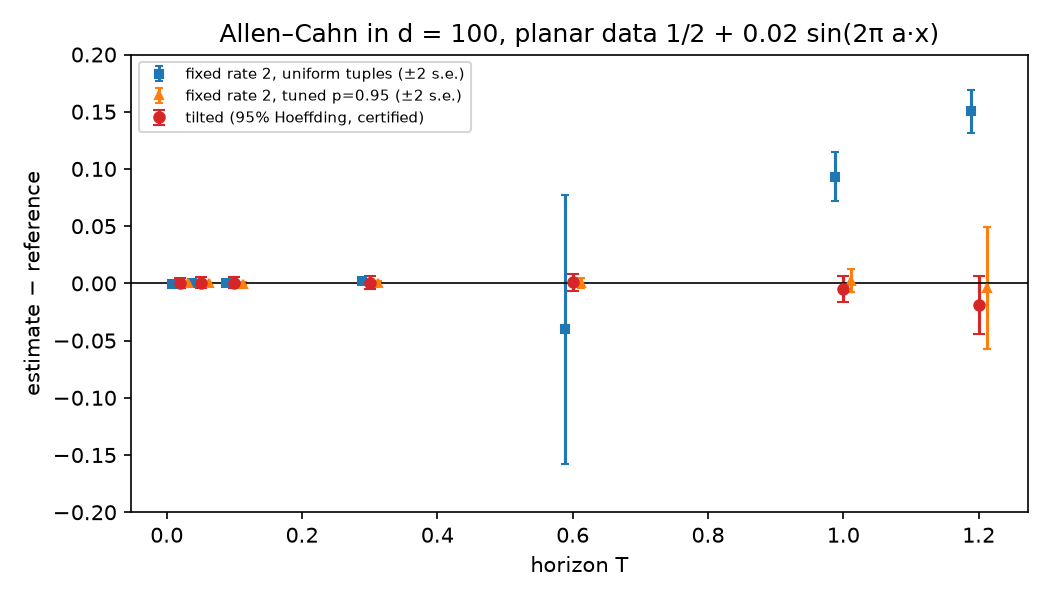
\includegraphics[width=0.8\textwidth]{tilted_high_dim.png}
\caption{Error of the estimates of $u(0,a/4)$ in dimension $100$.}
\label{fig:hd}
\end{figure}

\paragraph{A limitation.} For the traveling-wave data
$v(x)=-\frac12-\frac12\tanh(-x/2)$ of \cite{NPP23}, the range of $v$
is $(-1,0)$ and the sup envelopes combine the jets of $f$ near $-1$ and
near $0$; the guaranteed horizon is only $0.666$, and within it the
rate-one fixed sampler has a two to three times smaller product of
variance and work (with unbounded outputs). Spatially varying
supersolutions, as in Theorem~\ref{thm:E}, are needed for such data.

\section{Discussion}

The results separate three quantities that are often conflated: the
existence horizon of the PDE, the integrability horizon of a fixed
expansion, and the finite-variance horizon of a particular sampler. The
second is characterized by one positive system and cannot be improved by
sampling; the gap between the second and the third can be closed
completely, with bounded output and horizon-free expected work, whenever
a supersolution with slack is available. Extending the horizon beyond the
integrability horizon requires changing the expansion itself (e.g.\
time-patching \cite{Warin17,HP26} or bounded voting representations),
which is outside the scope of this paper. Open problems include
computable spatially varying supersolutions for general data, the
fully nonlinear mechanisms of \cite{NPP23}, and the endpoint work
frontier.

\appendix

\section{Proof of Proposition~\ref{prop:corr}}\label{app:corr}

Let $m=\deg f$. Codes $F_k$ with $k>m$ have $g_{F_k}\equiv0$ and every
tuple issued from them contains a code $F_{k'}$ with $k'>k$; by induction
on the depth, every finite tree rooted at such a code has $a=0$. The
remaining codes $\Id,F_0,\dots,F_m,D_1,\dots,D_d$ form a finite set, and by
Lemma~\ref{lem:majorant} the vector $Y=(U_c)_c$ is a mild solution on
$[0,T]$ of the finite signed system
\begin{equation}\label{eq:S}
Y_c(t)=P_tg_c+\sum_j\kappa_j\int_0^tP_{t-s}\Big[\prod_iY_{c_{j,i}}(s)\Big]\dd s,
\end{equation}
with $|Y_c|\le W_c\le M$ on $[0,T]\times\X$.

By standard semilinear parabolic theory in $BUC(\X)$ (locally Lipschitz
$f$), \eqref{eq:pde} has a unique mild solution $u$ on a maximal interval
$[0,T_{\max})$, with $\limsup_{t\uparrow T_{\max}}\|u(t)\|_\infty=\infty$
if $T_{\max}<\infty$. For $v\in C^2_b$ and polynomial $f$, $u$ is classical
on $(0,T_{\max})$, and on every $[0,t']$ with $t'<T_{\max}$ the functions
$u$, $\nabla u$ are bounded and continuous up to $t=0$; for $\nabla u$ this
follows from $\nabla u(t)=P_t\nabla v+\int_0^t\nabla P_{t-s}f(u(s))\dd s$
and $\|\nabla P_r\|_{\infty\to\infty}\le Cr^{-1/2}$. The chain rule gives
\[
(\partial_t-L)f^{(k)}(u)=f^{(k+1)}(u)f(u)-\tfrac12f^{(k+2)}(u)|\nabla u|^2,
\qquad (\partial_t-L)\partial_iu=f'(u)\partial_iu,
\]
so by Duhamel's formula for bounded classical solutions the physical
family $\tilde Y=(u,f^{(k)}(u),\partial_iu)$ solves \eqref{eq:S} on
$[0,t']$ with the same initial data.

The right-hand side of \eqref{eq:S} is a polynomial map, Lipschitz on
bounded subsets of $BUC(\X)^{|\C|}$ with a constant $\Lambda$. For
$t'<\min(T,T_{\max})$ both $Y$ and $\tilde Y$ are bounded on $[0,t']$, and
$\|Y(t)-\tilde Y(t)\|_\infty\le\Lambda\int_0^t\|Y(s)-\tilde Y(s)\|_\infty
\dd s$ with $P_{t-s}$ a contraction; Gronwall's lemma gives $Y=\tilde Y$.
In particular $\|u(t)\|_\infty=\|U_\Id(t)\|_\infty\le M$ on
$[0,\min(T,T_{\max}))$, so the blow-up alternative excludes
$T_{\max}\le T$. Hence $U_\Id=u$ on $[0,T]$. \qed

\section{Proof of Theorem~\ref{thm:D}: sufficiency and the
classification}\label{app:D}

Throughout, ``tree'' means a finite completed tree of
Example~\ref{ex:semilinear}, and $\X$ is connected.

\emph{(i) Higher jets vanish.} Suppose $f^{(p)}(v)\equiv0$ for all
$p\ge2$. We claim $a(\theta)=0$ for every tree rooted at $F_k$, $k\ge2$.
Induct on the depth: a leaf has $g_{F_k}=f^{(k)}(v)\equiv0$; a branch uses
$(F_0,F_{k+1})$ or $(D_i,D_i,F_{k+2})$, each containing a child $F_{k'}$
with $k'\ge3$, whose subtree has zero weight. Hence $W_{F_k}\equiv0$ for
$k\ge2$, and every tuple containing such a code contributes nothing.
Moreover $\nabla f'(v)=f''(v)\nabla v\equiv0$, so $f'(v)\equiv b$ is
constant on the connected space $\X$. The surviving part of
\eqref{eq:majorant} reads $W_{F_1}=P_t|b|=|b|$ and
$W_{F_0}(t)=P_t|f(v)|+|b|\int_0^tP_{t-s}W_{F_0}(s)\dd s$, whose minimal
solution is $e^{|b|t}P_t|f(v)|$. Therefore
\[
W_\Id(t)=P_t|v|+\frac{e^{|b|t}-1}{|b|}P_t|f(v)|
\qquad(\text{with }t\text{ in place of the fraction if }b=0),
\]
which is finite for all $t$.

\emph{(ii) $f(v)\equiv0$.} If $v$ is nonconstant, $v(\X)$ is a
nondegenerate interval on which $f$ vanishes, hence all derivatives
$f^{(k)}$ vanish on it and $g_{F_k}\equiv0$ for every $k$. Every tree rooted
at some $F_k$ has zero weight by induction on the depth (a leaf is zero; a
branch contains an $F$-child). Thus $W_{F_0}\equiv0$ and $W_\Id=P_t|v|$. If
$v\equiv r$ with $f(r)=0$, then $g_{F_0}=0$ and $g_{D_i}=0$; every tree
rooted at $D_i$ has zero weight (each branch $D_i\to(F_1,D_i)$ contains a
$D_i$-child), and every tree rooted at $F_0$ has zero weight (a branch
contains an $F_0$-child or a $D_i$-child). Again $W_\Id=|r|$.

\emph{(iii) Necessity.} If neither (i) nor (ii) holds, $f(v)\not\equiv0$
and $f^{(p)}(v)\not\equiv0$ for some $p\ge2$, and the obstruction proved
in Section~\ref{sec:explicit} applies. For completeness we record the
comparison step. The finite system $V_k=\eta_k\mathbf 1_{k\in\{0\}}+
\int_0^sV_0V_{k+1}$ ($0\le k<p$), $V_p\equiv\eta_p$, has
$V_{p-j}=\eta_pZ^j/j!$ for $1\le j\le p-1$ and
$V_0=\eta_0+\eta_pZ^p/p!$ with $Z'=V_0$, $Z(0)=0$; its Picard iterates
started at $0$ are dominated by $(A_k)$ by induction, since $A$
satisfies the same inequalities. Hence $A_0=\infty$ after the explosion
time $s_*=\int_0^\infty\dd z/(\eta_0+\eta_pz^p/p!)$, and splitting the
integral at $z_1=(\eta_0p!/\eta_p)^{1/p}$ gives
$s_*<z_1/\eta_0+p!/((p-1)\eta_pz_1^{p-1})=\frac p{p-1}\,z_1/\eta_0$, the
bound displayed in Theorem~\ref{thm:D}. Since
$W_\Id(T,x)\ge\int_0^TP_{T-r}W_{F_0}(r)(x)\dd r$ and $W_{F_0}=\infty$ on
$(t_0+s_*,\infty)\times\X$, $W_\Id(T,x)=\infty$ for $T>t_0+s_*$.

\emph{(iv) Classification.} (i)--(iii) prove the smooth statement. If
$f$ is real-analytic on an open interval $J\supset v(\X)$ and $v$ is
nonconstant, then $f''\equiv0$ on the nondegenerate interval $v(\X)$
implies $f$ affine on $J$ by the identity theorem, and $f(v)\equiv0$
implies $f\equiv0$ on $J$; conversely an affine $f$ satisfies (i). For
constant $v\equiv r$ the condition reads: $f(r)=0$, or $f$ is affine on
$J$. \qed

\section{Proof of Theorem~\ref{thm:E} for $d\le4$}\label{app:E}

Discard the nonnegative source $\sum_iD_i^2$ and let $A_*,B_*$ be the
minimal extended solutions of
\[
A_*=P_tA_0+\int_0^tP_{t-s}(A_*B_*)\dd s,\qquad
B_*=P_tB_0+2\int_0^tP_{t-s}A_*\dd s,
\]
$A_0=\varepsilon^2e^{-2|x|^2}$, $B_0=2\varepsilon e^{-|x|^2}$; then
$W_{F_0}\ge A_*$ and $W_{F_1}\ge B_*$. All Picard iterates, hence $A_*,B_*$,
are radial and radially nonincreasing (the heat semigroup, products and
sums preserve this).

\emph{Correlation.} For nonnegative radial nonincreasing $\phi,\psi$ and
$\ell>0$, $P_\ell(\phi\psi)(0)\ge P_\ell\phi(0)P_\ell\psi(0)$ (Chebyshev's
inequality for two nonincreasing functions of the radius of a centred
Gaussian; truncation and monotone convergence cover extended values).

\emph{Riccati barrier.} Fix $t_0\ge0$, $T>0$, and set
$a(s)=P_{T-s}A_*(t_0+s)(0)$, $b(s)=P_{T-s}B_*(t_0+s)(0)$ for $0\le s<T$.
Splitting the Volterra integrals at $t_0$ and using the correlation
inequality,
$a(s)\ge a(0)+\int_0^sab$ and $b(s)\ge2\int_0^sa$. With
$z(s)=\int_0^sa$ this gives $z'\ge\alpha+z^2$ for $\alpha=a(0)$, so $z$
is infinite before $\pi/(2\sqrt\alpha)$. If $\pi/(2\sqrt\alpha)<T$ the
$\Id$ integral at horizon $t_0+T$ diverges at the origin. It diverges at
every $x$ because $P_\ell h(x)\ge e^{-|x|^2/(2\ell)}P_\ell h(0)$ for even
nonnegative $h$ (pair $y$ with $-y$), with $\ell\ge T-\pi/(2\sqrt\alpha)>0$.

\emph{$d\le3$.} With $t_0=0$, $a(0)=\varepsilon^2(1+4T)^{-d/2}$, and the
condition $T>\frac{\pi}{2\varepsilon}(1+4T)^{d/4}$ holds for
$T\ge T_d=\max\{1,(\pi5^{d/4}/\varepsilon)^{4/(4-d)}\}$, since
$1+4T\le5T$ for $T\ge1$. Hence $W_\Id(t,x)=\infty$ for $t\ge T_d$.

\emph{$d=4$.} From the equations, $A_*(t)\ge P_tA_0$ and
$B_*(t)\ge2tP_tA_0$, so $A_*(t)\ge L_A(t):=P_tA_0+\int_0^tP_{t-s}
[2s(P_sA_0)^2]\dd s$, a Gaussian mixture of total mass
\[
M_L(t)=\frac{\varepsilon^2\pi^2}{4}+\frac{\varepsilon^4\pi^2}{128}
\Big[\log(1+4t)+\frac1{1+4t}-1\Big],
\]
every component of which has variance at most $t+\frac14$. Let
$K=1+512\pi^2/\varepsilon^4$, $t_0=(e^K-1)/4$ and $T=t_0+\frac14$. Then
$M_L(t_0)>4\pi^4$ and, since a unit-mass Gaussian of variance $q\le T$
has $P_T$-value at the origin at least $(4\pi T)^{-2}$,
$a(0)\ge P_TL_A(t_0)(0)\ge M_L(t_0)/(16\pi^2T^2)>\pi^2/(4T^2)$. The
Riccati barrier gives $W_\Id(t,x)=\infty$ for all
$t\ge t_0+T=(2e^K-1)/4$ and all $x$. \qed

\bibliographystyle{abbrvnat}
\bibliography{refs}
\end{document}
